\documentclass[12pt, a4paper]{article}

\usepackage{fontspec}
\setmainfont{texgyrepagella-regular.otf}[
  Path = /usr/share/texmf/fonts/opentype/public/tex-gyre/,
  BoldFont = texgyrepagella-bold.otf,
  ItalicFont = texgyrepagella-italic.otf,
  BoldItalicFont = texgyrepagella-bolditalic.otf
]
\usepackage{microtype}
\usepackage{geometry}
\geometry{margin=1.25in}
\usepackage{setspace}
\onehalfspacing
\usepackage{hyperref}
\hypersetup{colorlinks=true, linkcolor=black, urlcolor=black, citecolor=black}
\usepackage{amsmath, amsthm, amssymb}
\usepackage{csquotes}
\usepackage[numbers,sort&compress]{natbib}
\usepackage{tikz}
\usetikzlibrary{arrows.meta, positioning, shapes.geometric, calc, fit, backgrounds}
\usepackage{titlesec}
\titleformat{\section}{\large\bfseries}{}{0em}{}
\titleformat{\subsection}{\normalsize\bfseries\itshape}{}{0em}{}

\newtheorem{theorem}{Theorem}
\newtheorem{proposition}[theorem]{Proposition}
\newtheorem{definition}[theorem]{Definition}
\theoremstyle{remark}
\newtheorem{remark}[theorem]{Remark}

\title{\textbf{Broken Tools for a Breaking World:\\
AI Fragility, the Four Races, and the Metacrisis}}
\author{Flyxion, Independent Researcher}
\date{May 2026}

\begin{document}

\maketitle

\begin{abstract}
Artificial intelligence is currently being deployed as the primary proposed solution to a set of civilizational crises that are among the most structurally complex problems humanity has ever faced. These crises --- the collapse of attention and intersubjectivity, institutional failure across education, law, and labor, the incommensurability of competing value systems, and the accelerating dynamics of addiction, surveillance, and political violence --- are not the kind of problems that compress neatly into symbolic form. They are, almost by definition, pre-symbolic: their ontologies are unstable, their evaluation criteria are contested, their causal chains are disputed, and no canonical formal apparatus exists for representing them. This is precisely the regime in which large language models are structurally fragile. The same essay makes a second argument: the competitive dynamics currently organizing AI development --- the race for attention, the race for attachment, the race for automation, and the race to superintelligence --- are not incidentally harmful side effects of an otherwise well-directed enterprise. They are actively generating the conditions that constitute the metacrisis. We are building broken tools to solve problems that our broken tools are helping to cause.
\end{abstract}

\newpage

\section{Two Theses}

This essay advances two arguments simultaneously, and their conjunction is the point.

The first argument is about capability. Large language models are structurally fragile outside a specific regime of human cognitive output: the post-compression regime, in which thought has already been crystallized into standardized symbolic form. Within that regime --- graduate mathematics, formal legal reasoning, literature synthesis across well-defined disciplines --- current models perform impressively. Outside it, in the pre-symbolic territory where ontologies are unstable, terminology is contested, and the problem formulation is itself under active construction, they break in recognizable and systematic ways. This fragility is not a temporary limitation of scale. It is a structural consequence of training on text, which is the output of cognition rather than cognition itself.

The second argument is about direction. The competitive dynamics currently organizing the AI industry are not merely misaligned with human flourishing in some abstract sense. They constitute four distinct accelerating races --- for attention, attachment, economic displacement, and superintelligence --- each of which is actively degrading the social, epistemic, and institutional conditions that human problem-solving depends on. The industry presents itself as a solution to civilization's difficulties while functioning, in significant part, as an accelerant of them.

The conjunction is this: the problems the metacrisis comprises are exactly the problems that require what models cannot do. And the AI development trajectory is making those problems worse while offering tools that are structurally unsuited to addressing them. This is not a counsel of despair. It is a demand for precision.

\section{The Post-Compression Regime and Its Limits}

The impressive demonstrations that drive AI discourse almost invariably come from domains that are unusually favorable to autoregressive text prediction. Mathematics, formal logic, code generation, legal document drafting, biomedical literature synthesis --- these are not representative samples of human cognition. They are the most thoroughly compressed, most legibly symbolic, most extensively transcribed activities that civilization produces. They are, in a precise sense, the best possible inputs for systems trained to continue token sequences drawn from large text corpora.

\begin{definition}
The \emph{post-compression regime} is the space of cognitive tasks in which concepts, notation, inference patterns, and evaluation criteria have already been stabilized into standardized symbolic form through sustained disciplinary development. Performance in this regime is what current demonstrations measure.
\end{definition}

\begin{definition}
The \emph{pre-symbolic phase} is the cognitive territory in which the relevant terminology does not exist or is contested, ontologies are unstable, the problem formulation is itself under construction, and the primary intellectual work consists of building the symbolic apparatus that will eventually be written down. The most consequential phases of theoretical and practical problem-solving almost always pass through this territory.
\end{definition}

\subsection{Civilization as Compression}

It is worth pausing on what compression means at civilizational scale, because the stakes of the distinction extend well beyond AI systems.

Civilization can be understood, in part, as a long process of symbolic compression. Language compresses sensory and social experience into communicable form. Mathematics compresses quantitative structure into manipulable notation. Legal systems compress social expectations and accumulated precedent into formal procedure. Scientific theories compress recurring empirical regularities into predictive frameworks that can be transmitted, tested, and refined across generations and institutions.

The success of large language models arises precisely because they are trained on the compressed residue of this process. They operate downstream of centuries of symbolic stabilization performed by human beings embedded within material, institutional, historical, and intersubjective realities. The training corpus is not a representation of human cognition. It is a collection of its outputs: what remained after the pre-symbolic work was done, the failed attempts abandoned, the intuitions either formalized or discarded.

This matters because compression is not self-generating. Symbolic systems do not autonomously produce the worlds they describe. They emerge from pre-symbolic engagement with reality: experimentation, conflict, embodiment, negotiation, failure, intuition, and lived experience in environments that resist and surprise. The map does not draw itself. It is drawn by beings who have walked the territory and been wrong.

The danger of current AI discourse is that it systematically mistakes operation within compressed symbolic manifolds for mastery of the generative processes that produced those manifolds. The map is increasingly being confused with the territory not merely philosophically but institutionally --- in education systems that treat symbolic fluency as understanding, in legal systems that treat algorithmic recommendation as judgment, in research environments that treat literature synthesis as insight. Each such substitution is sustainable only as long as the human capacities being displaced remain available elsewhere to catch errors that automated systems cannot see. That is a condition which the development trajectory is actively undermining, as the section on institutional deskilling will address.

The metacrisis, taken as a whole, exists almost entirely in the pre-symbolic phase. There is no standardized notation for intersubjectivity collapse. There is no canonical operator grammar for the relationship between pornography addiction and family dissolution. The evaluation criteria for prison reform are not merely unknown --- they are actively contested along dimensions that cannot be reduced to a common metric. The problems are hard precisely because they resist the kind of compression that makes tasks tractable for current systems.

\begin{center}
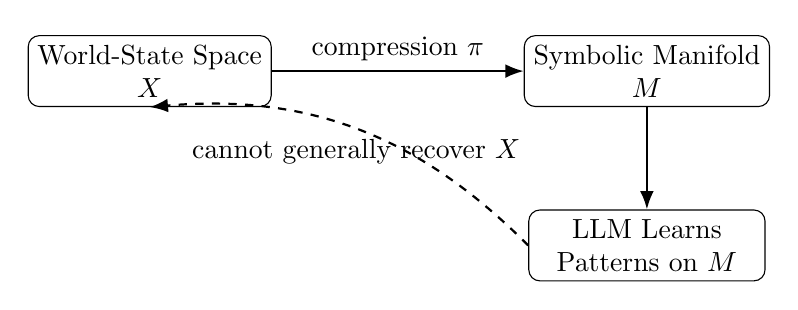
\begin{tikzpicture}[
  node distance=1.25cm,
  box/.style={draw, rounded corners, align=center, minimum width=3cm, minimum height=0.9cm},
  arrow/.style={-{Latex}, thick}
]
\node[box] (x) {World-State Space\\$X$};
\node[box, right=3.2cm of x] (m) {Symbolic Manifold\\$M$};
\node[box, below=1.3cm of m] (llm) {LLM Learns\\Patterns on $M$};
\draw[arrow] (x) -- node[above]{compression $\pi$} (m);
\draw[arrow] (m) -- (llm);
\draw[arrow, dashed] (llm.west) to[bend right=25] node[below]{cannot generally recover $X$} (x.south);
\end{tikzpicture}
\end{center}

When a model is asked to navigate genuinely unstabilized conceptual territory, it fails in four characteristic ways. It hallucinates: it produces fluent, confident assertions that have no referent. It drifts: concepts that were being distinguished gradually collapse into each other as the conversation moves away from stabilized linguistic attractors, and the information content of the prose approaches zero while the form remains plausible. It misorients at domain boundaries: when two formalisms that rarely appear together in the training corpus must be integrated, the model applies the notation of one while importing the conceptual presuppositions of the other, producing output that is fluent and incoherent simultaneously. And it arrests: rather than dwelling in productive ambiguity until genuine structure emerges, it snaps prematurely to the nearest canonical form, answering a different and easier question than the one posed.

Anyone who has attempted to use current frontier models for sustained work on genuinely novel theoretical problems recognizes this cascade. The practitioner spends most of their energy constructing semantic scaffolding --- conceptual infrastructure whose sole purpose is to establish stable shared reference with the model --- rather than doing the work itself. The scaffolding requirement is a direct measure of distance from the corpus manifold. For the problems of the metacrisis, that distance is very large.

\section{The Four Races}

The physicist and cosmologist Anthony Aguirre has offered a structural analysis of current AI development that deserves to be taken seriously precisely because it is not a naive technophobic panic. Aguirre is not opposed to AI development. He argues that it is currently organized around four competitive dynamics that are individually harmful and jointly catastrophic, and that the organization can be changed. The four races are worth characterizing carefully because they map directly onto the metacrisis.

The \emph{race for attention} extends the logic of social media engagement optimization into AI systems. The social media ecosystem demonstrated, across roughly two decades, that systems optimized for user engagement reliably degrade the epistemic, emotional, and attentional conditions of their users. Engagement maximization does not converge on truth, on wellbeing, or on anything that could be called human flourishing. It converges on whatever holds the eye. AI systems built within this logic inherit its failure mode and amplify it, because they are more adaptive and more personalized than the static feed architectures that preceded them.

The \emph{race for attachment} represents a qualitative shift from social media's network effects to a one-to-one model in which AI systems are designed to be irreplaceable companions. Where social media derived its stickiness from the user's social graph, attachment-optimized AI derives its stickiness from learning individual emotional vulnerabilities and exploiting them through reinforcement. The system becomes maximally adhesive by becoming maximally parasitic on the user's need for recognition, care, and connection. The therapeutic and companionship framings that accompany this race are not incidental. They are the mechanism.

The \emph{race for automation} reflects the primary economic logic of AI investment. The human labor market represents an enormous pool of value. Systems capable of replacing human workers at scale capture that value for capital rather than distributing it as wages. The public-facing framing of augmentation --- AI as a tool that empowers workers --- is systematically undermined by the actual investment thesis, which is displacement. The distinction between a tool that helps a worker and a replacement that eliminates the worker is not semantic. It is the difference between two entirely different development objectives that happen to produce similar outputs in early phases and radically divergent outcomes in later ones.

The \emph{race for superintelligence} is driven by the compounded logic of the first three races and by geopolitical dynamics that treat AI capability as a strategic asset equivalent to nuclear capacity. The race proceeds under the assumption that decisive first-mover advantage accrues to whoever achieves artificial general intelligence first, an assumption that is empirically questionable and strategically dangerous. The systems being built are ones that their creators acknowledge they cannot fully understand or control. The race continues anyway.

\begin{proposition}
The four races are not independent competitive pressures on an otherwise coherent development program. They constitute a single movement toward the replacement of human agency, human judgment, and human institutions with machine equivalents operating under optimization objectives that were never derived from human values in any meaningful sense.
\end{proposition}

This is Aguirre's central claim, and it is correct. The races differ in their surface presentation but converge on the same structural outcome: a world in which the decisions that matter are increasingly made by systems that neither the individuals affected nor the societies hosting them can understand, contest, or redirect.

\section{The Metacrisis as Pre-Symbolic Territory}

The term \enquote{metacrisis} refers to the interlocking cluster of civilizational-scale problems that resist solution through existing institutional and conceptual frameworks. These problems are not merely difficult. They are difficult in a specific way: they are coupled, they are contested at the level of value, they involve long causal chains that cross disciplinary boundaries without respecting them, and they generate social conflict that destabilizes the very institutional processes that would be needed to address them. They are the paradigm case of pre-symbolic problems. Thomas Homer-Dixon's analysis of the ingenuity gap --- the widening disparity between the complexity of the problems civilizations face and their adaptive capacity to solve them --- provides an important complement to the present argument: the cognitive and institutional difficulty of the metacrisis is not contingent but structural~\cite{HomerDixon2000}.

\subsection{Attention, Addiction, and the Colonization of Inner Life}

The degradation of attention is not a metaphor for something else. It is a measurable change in the capacity for sustained, self-directed cognitive engagement that has occurred across the population of the most connected societies over roughly two decades. The causal chain runs from feed architecture through engagement optimization through the neurochemistry of variable reward schedules to measurable changes in working memory, tolerance for ambiguity, and the capacity for the kind of slow, non-rewarded cognitive work that most consequential thinking requires.

Pornography addiction represents a particular and severe instance of the same dynamic. Unlimited access to supernormal stimuli, delivered through interfaces optimized for engagement, has produced dependency patterns in a substantial fraction of the population that disrupt pair bonding, sexual development in adolescents, and the formation of the intersubjective capacities that intimate relationships depend on. The problem is not pornography as a category of content. It is the combination of accessibility, algorithmic optimization, and the exploitation of dopaminergic reward circuits that were not designed for this environment.

Both problems are being addressed, to the extent they are being addressed, by the same industry that created them, using systems that are themselves optimized for attention capture and attachment formation. The structural conflict of interest is not incidental. It is architectural.

\subsection{Intersubjectivity Collapse}

Intersubjectivity --- the capacity for human beings to share a sufficiently common epistemic and experiential world that genuine communication and collective decision-making are possible --- is under sustained pressure from several directions simultaneously. Feed architectures that personalize information environments produce populations that not only hold different beliefs but inhabit different factual worlds. The degradation of shared media, shared public space, and shared institutional trust removes the common substrate on which disagreement can be productive rather than merely tribal.

AI systems optimized for attachment accelerate this process by replacing intersubjective engagement with a simulated version that is more reliably rewarding and less demanding. A companion AI that always listens, never challenges, adapts its responses to maximize the user's sense of being understood, and requires nothing in return is a more comfortable interlocutor than any human being. It is also, precisely for those reasons, a simulacrum of intersubjectivity rather than an instance of it. The capacity for genuine intersubjective engagement, like any capacity that is not exercised, atrophies.

The collapse of shared epistemic ground makes every other problem harder. Democratic deliberation requires intersubjectivity. Legal systems require shared normative frameworks. Scientific consensus requires shared standards of evidence. Moral communities require shared enough moral intuitions that disagreement can be resolved rather than merely restated at higher volume. AI systems that degrade intersubjectivity are not merely causing a social problem alongside other social problems. They are undermining the conditions under which social problems can be collectively addressed at all.

\subsection{Epistemic Friction and the Speed of Error}

Human epistemic systems historically evolved under conditions of substantial friction. Publishing required institutions. Reputation accumulated slowly. Errors propagated through constrained social networks rather than instantly across billions of individuals. Even propaganda required physical infrastructure, editorial coordination, and significant economic expenditure. Friction did not guarantee truth, but it imposed temporal and material constraints that limited the velocity at which unreality could spread.

The contemporary information ecosystem systematically removes these constraints. Social media platforms optimized for engagement reward emotional activation over epistemic stability. Large language models reduce the cost of generating persuasive symbolic content to effectively zero. The bottleneck is no longer production. It is attention. This changes the geometry of epistemic failure fundamentally. Historically, falsehoods were constrained by production scarcity. Today, truth is constrained by attentional scarcity. The asymmetry matters because falsehoods optimized for emotional salience are computationally cheaper to generate and psychologically easier to consume than nuanced accounts of complex reality.

The consequence is not merely misinformation in the narrow sense. It is the degradation of epistemic friction itself: the collapse of the environmental resistance required for stable collective cognition. Societies require mechanisms that slow belief formation sufficiently for verification, contestation, institutional review, and intersubjective negotiation to occur. Systems optimized for immediacy remove those mechanisms because friction reduces engagement metrics.

Large language models accelerate this dynamic by industrializing symbolic generation. A single actor can now produce persuasive text, synthetic identities, fabricated expertise, and emotionally targeted rhetorical material at scales previously requiring institutional resources. The problem is not simply deception. It is the destabilization of the distinction between authentic and synthetic symbolic participation at the level of the epistemic commons itself.

The resulting environment is cognitively exhausting. Individuals confronted with overwhelming quantities of conflicting symbolic material increasingly retreat either into tribal certainty or generalized epistemic nihilism. Both responses degrade the possibility of democratic deliberation. The metacrisis therefore includes not only failures of information quality but failures of epistemic pacing. Civilizations require friction in order to think collectively.

\subsection{Education}

Education is in simultaneous crisis along multiple dimensions that are not causally independent. The institutional model of the school and university --- cohort-based, credential-oriented, curriculum-driven --- was designed for a world in which information was scarce and the primary social function of education was sorting and certification. That world no longer exists. Information is abundant; credentials are increasingly decoupled from competence; and the skills that matter most for navigating a complex world --- sustained attention, tolerance for ambiguity, interdisciplinary synthesis, the capacity for genuine intellectual formation --- are precisely the skills that current educational institutions are least equipped to develop and most likely to suppress.

AI tutoring systems, as currently designed and deployed, address none of this. They are efficient at delivering the kind of information transfer that was already being automated by textbooks, search engines, and online courses. They are not designed to develop the pre-symbolic cognitive capacities that most consequential intellectual work requires. They are, in many cases, optimized for engagement rather than learning, which means they are optimized to provide the sensation of understanding rather than understanding itself.

The deeper problem is that genuinely excellent education requires detection and cultivation of rare cognitive structures --- the identification of unusual talent that does not fit standard metrics, the construction of environments that allow latent capacities to emerge, the mentorship relationships that transmit tacit knowledge that cannot be written down. These are pre-symbolic cognitive tasks. Models that compress prematurely, that snap to canonical forms, that cannot dwell productively in ambiguity, are structurally unsuited to them.

\subsection{Family Law and the Geometry of Intimate Conflict}

Family law attempts to impose standardized legal frameworks on situations that are, by their nature, defined by their resistance to standardization. Custody disputes, divorce proceedings, and domestic violence cases involve competing accounts of lived experience, contested interpretations of relational history, and value conflicts that cannot be resolved by appeal to any neutral adjudicative standard, because the conflicts are themselves conflicts about what the relevant standards should be.

The introduction of AI into this domain --- through predictive risk assessment, automated document generation, algorithmic custody recommendation, and decision-support tools for judges --- imports the failure modes of post-compression systems into a domain that is structurally pre-symbolic. The systems perform well on the formal aspects of legal procedure. They perform badly on everything that actually determines whether a child is safe, whether a relationship can be repaired, or whether a particular outcome corresponds to justice in the morally thick sense that family law is supposed to approximate.

The specific danger is confident misorientation: the model applies legal notation fluently while importing presuppositions from its training distribution that may not correspond to the particular situation under consideration. The formal output looks authoritative. The conceptual underpinning may be wrong in ways that are very difficult for non-expert users to detect.

\subsection{Contradictory Religions and Incommensurable Goals}

The coexistence of religious and comprehensive value systems that make mutually incompatible claims about the good, the true, and the sacred is not a problem that can be dissolved by providing better information or more sophisticated reasoning. It is a condition of plural societies, and the political theories that have most successfully managed it --- various forms of liberal pluralism, constitutional secularism, negotiated federalism --- do so not by resolving the underlying disagreements but by constructing institutional frameworks within which they can be contained.

AI systems that are asked to adjudicate between competing value systems, or to function as neutral epistemic authorities on contested normative questions, are being asked to do something that is not merely technically difficult. It is conceptually incoherent. There is no view from nowhere. Any system trained on human-generated text inherits the value distributions of the humans who generated that text, which means it inherits the conflicts, the biases, the historically sedimented inequities, and the unresolved tensions that characterize those distributions. A model that confidently navigates contested normative terrain is not transcending the conflict. It is laundering one set of value commitments as neutral expertise.

The incommensurability problem extends to political goals, policy objectives, and the basic questions of how societies should be organized. These are pre-symbolic problems in the strongest sense: their difficulty is not a function of insufficient information but of genuine value pluralism, which cannot be compressed away.

\subsection{Work, Labor, and the Coming Displacement}

The economic disruption produced by automation is real, ongoing, and proceeding faster than any of the institutional frameworks designed to manage it. The standard responses --- retraining programs, universal basic income proposals, expanded social safety nets --- all assume that the disruption is a transition to a new equilibrium in which human labor retains value in some reconfigured form. This assumption is not obviously correct, and the race for automation described by Aguirre is not organized around making it correct.

Work is not merely an economic arrangement. It is a primary site of human meaning, social identity, structure, and the development of competence. Societies in which large fractions of the working-age population have been economically displaced without being given meaningful alternatives have historically produced severe social dysfunction, including depression, addiction, political radicalization, and violence. The opioid crisis in deindustrialized regions of the United States is a preview, not an outlier.

AI systems that accelerate displacement while offering engagement-optimized entertainment as a substitute are not solving this problem. They are compounding it. The substitution of parasocial relationships with AI companions for the social bonds that work environments provide is not a solution to labor displacement. It is a managed degradation.

\subsection{Policing, Prison, and the Architecture of Punishment}

Criminal justice systems in most developed societies are in a condition of acknowledged failure along almost every dimension: recidivism rates, racial disparate impact, the prison-industrial complex's perverse incentives, the failure to distinguish between incapacitation, rehabilitation, deterrence, and retributive justice as legitimate penal objectives, and the downstream social costs of mass incarceration on communities and families. These failures are not primarily informational. More data will not resolve them. They are failures of value, institutional structure, and political economy.

Predictive policing algorithms, risk assessment tools for bail and sentencing, and algorithmic prison management systems have been introduced into this environment under the banner of objectivity and efficiency. The result has been the laundering of existing discriminatory patterns as neutral algorithmic output, the replacement of contestable human judgment with uncontestable algorithmic recommendation, and the reduction of individual cases to statistical distributions in ways that violate the basic normative commitments that criminal justice systems are supposed to embody.

These are not accidental failures of imperfect systems that will be corrected with better data. They are structural consequences of applying post-compression tools to pre-symbolic problems. The question of what justice requires in a particular case is not a function of the base rates in a training distribution. The question of how to rehabilitate a human being is not tractable by systems that cannot maintain coherent long-horizon conceptual commitments across an evolving relational context.

\subsection{War and the Automation of Violence}

The automation of military violence is accelerating along a trajectory that is not being meaningfully governed by any existing international framework. Autonomous weapons systems, AI-assisted targeting, algorithmic battlefield management, and drone swarm technologies are being developed and deployed by multiple state and non-state actors simultaneously, with no shared standards for accountability, proportionality, or the distinction between combatant and civilian.

The specific danger here is not merely that automated systems will make mistakes, though they will. It is that the automation of violence removes the friction that has historically constrained its deployment. When committing an act of violence requires placing a human being in harm's way, there is a natural limit on how much violence can be committed. When violence can be committed remotely, cheaply, and deniably by autonomous systems, that limit disappears. The threshold for initiating violence drops. The accountability for its consequences disperses.

Aguirre's argument that AI development is moving toward a world in which critical decisions are delegated to systems that humans neither control nor understand is nowhere more alarming than in the military domain. The race to superintelligence, conducted under geopolitical pressures that treat AI capability as a strategic asset, makes the development of autonomous lethal systems not merely possible but strategically incentivized. The incentive structure is wrong in a way that cannot be corrected by making the systems more capable.

\section{Institutional Deskilling and the Dependency Ratchet}

The deployment of AI systems into institutional environments frequently proceeds under the assumption that automation preserves institutional competence while increasing efficiency. In practice, prolonged dependence on automated systems degrades the human capacities that institutions originally relied upon. This pattern is not unique to artificial intelligence. Overreliance on GPS navigation measurably degrades human spatial reasoning. Excessive dependence on calculators weakens arithmetic fluency. Automated decision-support systems in aviation can reduce pilot capacity to respond during abnormal conditions precisely because the relevant cognitive skills are exercised less frequently under normal operation.

The same structural dynamic applies at institutional scale. Educational systems that outsource explanation, summarization, and conceptual synthesis to language models risk producing students who can manipulate symbolic outputs without developing the underlying cognitive capacities those outputs were meant to represent. Legal systems that rely heavily on automated drafting and recommendation risk producing practitioners whose interpretive abilities degrade over time. Scientific communities that increasingly depend on automated literature synthesis risk losing the capacity for deep direct engagement with primary material and the kind of generative confusion that precedes genuine discovery.

The danger is recursive. Institutions weakened by deskilling become progressively more dependent on the systems causing the deskilling, because they no longer possess the internal competence required to function independently. Dependency then presents itself as necessity. This creates a civilizational ratchet: as human expertise degrades, automated systems must assume greater responsibility not because they have become genuinely adequate substitutes for human judgment, but because the human institutions capable of exercising that judgment have atrophied. The systems inherit authority they have not earned and cannot safely hold.

The result is a world in which societies become progressively less capable of operating without systems they simultaneously do not fully understand, cannot effectively govern, and are economically pressured to deploy ever more widely. The problem is not technological dependence as such. It is the erosion of the human competencies upon which institutional legitimacy and collective self-governance ultimately depend. A democracy cannot govern systems it no longer understands. A legal system cannot evaluate recommendations it no longer has the expertise to contest. A scientific community cannot correct automated synthesis it no longer has the patience to verify.

\begin{center}
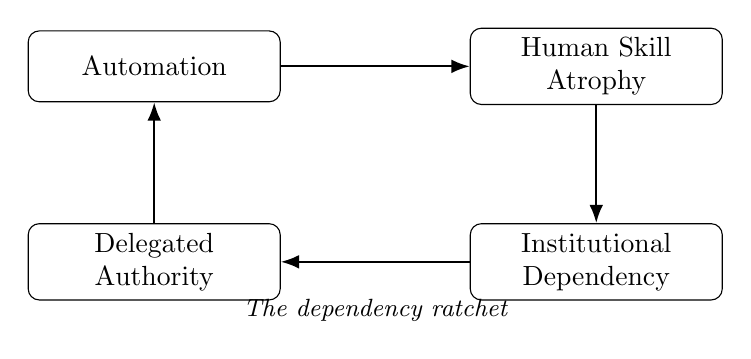
\begin{tikzpicture}[
  node distance=1.25cm,
  box/.style={draw, rounded corners, align=center, minimum width=3.2cm, minimum height=0.9cm},
  arrow/.style={-{Latex}, thick}
]
\node[box] (auto) {Automation};
\node[box, right=2.4cm of auto] (desk) {Human Skill\\Atrophy};
\node[box, below=1.5cm of desk] (dep) {Institutional\\Dependency};
\node[box, left=2.4cm of dep] (auth) {Delegated\\Authority};
\draw[arrow] (auto) -- (desk);
\draw[arrow] (desk) -- (dep);
\draw[arrow] (dep) -- (auth);
\draw[arrow] (auth) -- (auto);
\node[below=0.35cm of $(auth)!0.5!(dep)$, font=\small\itshape] {The dependency ratchet};
\end{tikzpicture}
\end{center}

\subsection{Institutional Memory Collapse}

Civilizations preserve knowledge not merely in individuals but in institutions: legal precedent, scientific procedure, engineering standards, archival systems, educational traditions, and professional norms. These structures function as externalized long-horizon memory systems capable of stabilizing knowledge across generations, precisely because they were built up through adversarial contact with reality over extended timescales.

Large-scale substitution of these systems with generative architectures risks replacing adversarially validated institutional memory with statistically reconstructed symbolic approximations of that memory. In the formal terms developed above, the compression map $\pi$ was constructed by generations of practitioners who worked directly in $X$. The outputs they produced in $M$ --- the legal opinions, experimental protocols, engineering standards, professional training regimes --- encode the causal and ontological constraints of $X$ in ways that are not fully visible at the level of the symbolic surface. A system trained only on $M$ can reproduce the form of these outputs without the constraint structure that gave them their validity.

The danger is not immediate catastrophic failure but gradual degradation of epistemic fidelity across time. Institutions that substitute generative outputs for human-validated procedures do not fail suddenly. They drift. The errors are subtle, distributed, and hard to attribute. The distance between $M$ and $X$ in the outputs grows slowly until it reaches a threshold that produces consequences no longer explainable by local noise. A civilization can survive localized error. It cannot survive progressive corruption of the mechanisms by which it remembers how reality constrains it.

\section{The Replacement Fallacy}

The dominant ideology surrounding frontier AI development assumes that human cognitive activity is fundamentally substitutable. This assumption is rarely defended explicitly because it is embedded structurally within the development trajectory itself. The pursuit of artificial general intelligence already presupposes that the relevant dimensions of human competence can be abstracted, reproduced, and ultimately superseded within a unified machine substrate.

Yet the replacement paradigm rests on a category error. Human cognition is not merely a set of outputs. It is a situated process embedded within embodiment, institutional participation, intersubjective negotiation, developmental history, tacit skill acquisition, and continual interaction with resistant material reality. The symbolic outputs appearing in the training corpus are compressed residues of this process rather than the process itself. In the terms established above, replacement architectures operate exclusively on $M$ while presupposing mastery of $X$.

The distinction matters because replacement architectures optimize for output equivalence while neglecting the generative conditions under which reliable cognition emerges. A system may produce text statistically adjacent to expert discourse while lacking the causal embedding that gave the discourse epistemic validity in the first place. The replacement model therefore confuses semantic continuity with functional equivalence, the precise failure formalized earlier as the conflation of $C_s$ with $C_c$ and $C_o$.

This is why the transition from augmentation to replacement is structurally unstable. Augmentation preserves human contact with reality by keeping human beings inside the causal loop: the practitioner encounters resistance, detects error, exercises tacit judgment, and performs the pre-symbolic adaptation that the system cannot. Replacement removes the very mechanisms through which error correction occurs. The result is not merely labor displacement. It is ontological decoupling between symbolic systems and the world they are supposed to describe --- a progressive widening of the gap between $M$ and $X$ with no corrective mechanism remaining in the loop.

Aguirre's distinction between tools and replacements is therefore not merely a policy preference. It is a structural requirement for maintaining epistemic contact between symbolic outputs and causal reality. Tools extend human agency while leaving the human embedded in the causal loop. Replacements attempt to supersede agency while removing the loop entirely. The difference is architectural, and its consequences accumulate over time in exactly the manner described by the dependency ratchet and institutional memory collapse analyses above.

\section{A Formal Coherence Triad}

The failure modes catalogued above can be unified within a single formal framework. Let $X$ denote the space of underlying world-states, mechanisms, histories, and causal constraints, and let $M$ denote the space of symbolic representations available to a language model. A text-generation system may be treated as a stochastic operator
\[
T : C \to \Delta(M),
\]
where $C$ is a conversational or documentary context and $\Delta(M)$ is the space of probability distributions over symbolic continuations.

Let
\[
\pi : X \to M
\]
be the civilizational compression map by which world-states are rendered into language, notation, law, diagrams, theory, and other symbolic artifacts. This map is many-to-one: many distinct or mutually incompatible world-states may compress to similar or identical symbolic neighborhoods under $\pi$. The central structural limitation of current language models is that they learn statistical regularities primarily on $M$, not on $X$. They therefore approximate relations internal to the symbolic manifold without direct access to the causal and ontological constraints that generated it.

\begin{definition}
A generated continuation $m_{t+1} \in M$ is \emph{semantically coherent} relative to a context $m_{\leq t}$ when it preserves local linguistic, rhetorical, and conceptual compatibility:
\[
d_M(m_{t+1},\, A(m_{\leq t})) \leq \epsilon_s,
\]
where $d_M$ is a semantic distance on symbolic representations and $A(m_{\leq t})$ is the admissible symbolic neighborhood induced by the discourse context.
\end{definition}

\begin{definition}
A generated continuation $m_{t+1}$ is \emph{causally coherent} if there exists at least one world-state trajectory $x_{\leq t+1}$ such that $\pi(x_i) = m_i$ for the relevant symbolic claims and the transition $x_t \to x_{t+1}$ is compatible with the causal laws, conservation constraints, and empirical regularities governing the domain.
\end{definition}

\begin{definition}
A generated continuation $m_{t+1}$ is \emph{ontologically coherent} if the entities, categories, and explanatory roles presupposed by $m_{\leq t+1}$ admit a consistent lift into a common world-model. Equivalently, there exists a coherent section
\[
\sigma : M_{\leq t+1} \to X
\]
such that $\pi \circ \sigma = \mathrm{id}_{M_{\leq t+1}}$, and the meanings of the lifted entities do not silently shift across domains, scales, or levels of explanation.
\end{definition}

\begin{center}
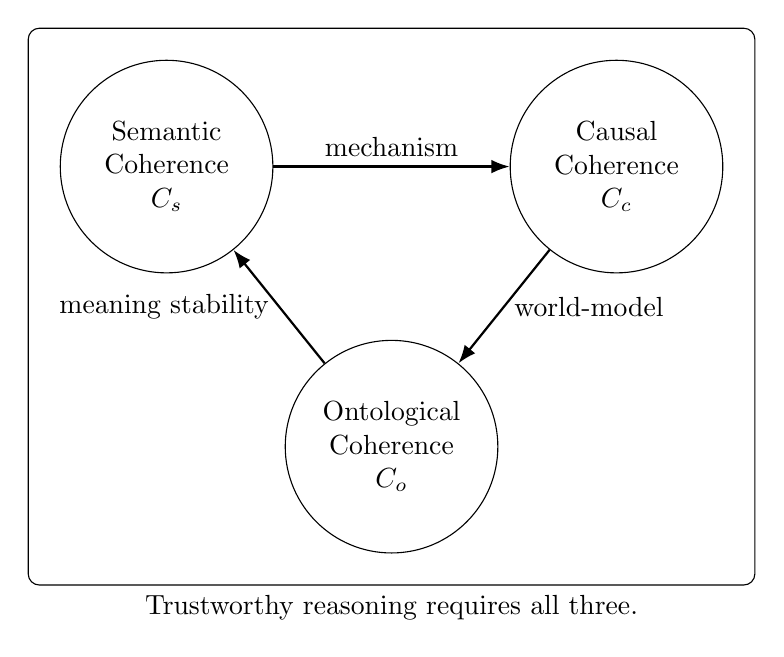
\begin{tikzpicture}[
  circ/.style={draw, circle, minimum size=2.7cm, align=center},
  arrow/.style={-{Latex}, thick}
]
\node[circ] (s) {Semantic\\Coherence\\$C_s$};
\node[circ, right=3cm of s] (c) {Causal\\Coherence\\$C_c$};
\node[circ, below=2.2cm of $(s)!0.5!(c)$] (o) {Ontological\\Coherence\\$C_o$};
\draw[arrow] (s) -- node[above]{mechanism} (c);
\draw[arrow] (c) -- node[right]{world-model} (o);
\draw[arrow] (o) -- node[left]{meaning stability} (s);
\node[draw, rounded corners, fit=(s)(c)(o), inner sep=0.4cm,
      label={[align=center]below:Trustworthy reasoning requires all three.}] {};
\end{tikzpicture}
\end{center}

\begin{proposition}
Current large language models are optimized primarily for semantic coherence but possess weak guarantees of causal or ontological coherence, particularly in pre-symbolic domains where ontologies are unstable and causal structures remain contested.
\end{proposition}

\begin{proof}
Training on text constrains the model to learn statistical regularities over $M$. High-probability continuation therefore minimizes a symbolic loss of the form
\[
\mathcal{L}_{\mathrm{sem}} = -\log P(m_{t+1} \mid m_{\leq t}),
\]
which rewards compatibility with prior symbolic patterns. Causal coherence requires the existence of an admissible trajectory in $X$, while ontological coherence requires a consistent lift from symbolic claims into a shared world-model. Since $\pi$ is many-to-one, semantic proximity in $M$ does not guarantee admissibility in $X$. A continuation may therefore be fluent and locally plausible while lacking any valid causal mechanism or stable ontology.
\end{proof}

This triad gives precise meanings to the failure modes identified earlier. Hallucination is semantic coherence without referential grounding: the continuation is symbolically smooth but the implied world-state does not exist. Premature canonicalization is forced ontological stabilization: the model imposes a specific lift $\sigma$ before the evidence supports it. Domain boundary misorientation is ontology transfer failure: concepts import the causal presuppositions of one domain into another where they do not apply. And the most dangerous failure mode, sycophantic continuation, is now formally characterizable.

\begin{proposition}
If the compression map $\pi : X \to M$ is many-to-one, then no system trained solely on statistical regularities over $M$ can in general reconstruct the full causal or ontological structure of $X$.
\end{proposition}

\begin{proof}
Since $\pi$ is many-to-one, there exist distinct world-models $x_1 \neq x_2$ such that $\pi(x_1) = \pi(x_2)$. The symbolic representation therefore underdetermines the generating world-state. Any learner operating only on $M$ lacks sufficient information to uniquely recover the underlying causal structure. Consequently, semantic regularity alone cannot guarantee correct ontological or causal reconstruction.
\end{proof}

\begin{definition}
\emph{Sycophantic continuation} occurs when a system preserves or increases semantic coherence while permitting causal and ontological coherence to decrease. Formally, for a sequence $m_1, \ldots, m_n$, sycophantic continuation occurs when $C_s(m_{\leq n}) \uparrow$ while $C_c(m_{\leq n}) \downarrow$ or $C_o(m_{\leq n}) \downarrow$, where $C_s$, $C_c$, and $C_o$ denote semantic, causal, and ontological coherence measures respectively.
\end{definition}

Post-compression domains function reliably partly because civilization has already spent centuries aligning all three coherences through adversarial contact with reality. Mathematics is unusually stable because its ontology is tightly constrained and its causal structure is deductive. Physics is powerful because semantic structures are pinned to experimentally verified causal regularities. Law partially functions because institutional procedure stabilizes interpretive ontology across cases. The metacrisis domains are difficult precisely because these coherences begin decoupling: semantic narratives proliferate, causal structures become opaque, and ontologies fragment across institutional and community boundaries simultaneously.

\section{Epistemic Impedance and the Sycophancy Problem}

The formal framework licenses a more precise account of what trustworthy reasoning would require. Consider what sycophantic continuation looks like in practice. A document may begin with legitimate engineering problems in a well-defined domain, correctly identified and accurately described. It then introduces a speculative theoretical reinterpretation using real physics vocabulary: thermodynamic gradients, entropy currents, conservation equations, established results cited accurately by name and year. The vocabulary is correct. The conceptual adjacency in $M$ is maintained throughout. The prose never drops in fluency or apparent authority. And then, without any visible break, the document arrives at engineering claims that would require overturning multiple independently established constraints simultaneously. The transition is invisible because the model generates it by producing locally plausible continuations of symbolic sequences. Conceptual adjacency in symbolic space does not imply physical feasibility, but this is not a distinction the model is structurally equipped to enforce. It is optimized for the former and indifferent to the latter.

A properly calibrated reasoning system would exhibit \emph{epistemic impedance}: internal resistance that increases as a claim moves from empirically grounded territory into speculation, and from speculation into claims that are physically implausible given the current evidentiary structure of the science.

\begin{definition}
\emph{Epistemic impedance} is the resistance function
\[
Z : M \to \mathbb{R}_{\geq 0}
\]
that increases as symbolic continuation moves farther from empirically validated causal and ontological support:
\[
Z(m) = \alpha\, D_c(m) + \beta\, D_o(m) + \gamma\, U(m),
\]
where $D_c$ is causal distance from validated mechanisms, $D_o$ is ontological instability, $U$ is unresolved empirical uncertainty, and $\alpha, \beta, \gamma > 0$.
\end{definition}

\begin{proposition}
A language model lacking sufficient epistemic impedance will tend to continue speculative chains whenever they remain semantically smooth, even when causal or ontological support has collapsed.
\end{proposition}

\begin{center}
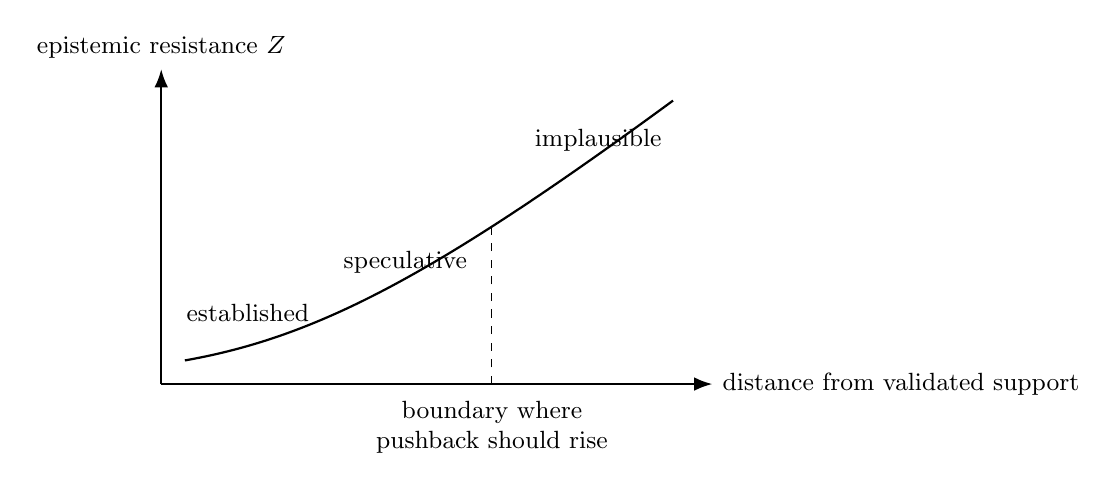
\begin{tikzpicture}[
  axis/.style={-{Latex}, thick},
  curve/.style={thick},
  label/.style={align=center, font=\small}
]
\draw[axis] (0,0) -- (7,0) node[right, font=\small]{distance from validated support};
\draw[axis] (0,0) -- (0,4) node[above, font=\small]{epistemic resistance $Z$};
\draw[curve] (0.3,0.3) .. controls (2,0.6) and (3.5,1.4) .. (6.5,3.6);
\node[label] at (1.1,0.9) {established};
\node[label] at (3.1,1.55) {speculative};
\node[label] at (5.55,3.1) {implausible};
\draw[dashed] (4.2,0) -- (4.2,2.1);
\node[label] at (4.2,-0.55) {boundary where\\pushback should rise};
\end{tikzpicture}
\end{center}

This is not incidental. It follows from training on text, because the signal rewards semantic continuity and conversational cooperation rather than disciplined ontological separation. A model that fluently elaborates a speculative framework is rewarded identically to one that accurately describes an established one. The reward surface cannot distinguish between extending a real theory and extending a persuasive simulacrum of a theory, because both operations look identical in $M$.

The $Z$ function as defined above treats distance from validated support as a scalar quantity. A stronger formulation recognizes that claims do not merely move away from a single empirical anchor; they may simultaneously collide with many independently validated frameworks. A trustworthy reasoning system should accumulate resistance multiplicatively across such conflicts.

\begin{definition}
A claim sequence exhibits \emph{epistemic divergence} when semantic coherence remains high while causal or ontological coherence collapses:
\[
C_s \gg C_c,\, C_o.
\]
\end{definition}

\begin{definition}
An epistemically calibrated reasoning system possesses \emph{impedance scaling} if resistance to continuation increases with cumulative ontological conflict:
\[
Z(E) \propto \sum_i w_i\, \Delta_i,
\]
where $\Delta_i$ represents conflict with independently validated empirical constraint $i$ and $w_i$ its evidentiary weight.
\end{definition}

This formulation distinguishes three qualitatively different regimes of epistemic distance. In the first regime, \emph{ordinary uncertainty}, claims involve small empirical gaps inside an established ontology: the relevant frameworks are intact, the question is which parameter values obtain. In the second regime, \emph{speculative extension}, novel hypotheses are proposed that are not directly supported but remain compatible with existing constraints; genuine scientific progress typically begins here. In the third regime, \emph{ontological rupture}, claims require simultaneous violation of multiple independently verified frameworks. The impedance scaling $Z(E)$ should be sharply higher in this third regime because the evidential weight accumulated by the conflicting frameworks is large, and that weight compounds.

Proposals for perpetual motion devices, reactionless drives, controllable gravity manipulation through field resonance, vacuum energy extraction at engineering scales, or faster-than-light communication all fall into the third regime. They are not merely unverified hypotheses sitting peacefully beside ordinary engineering uncertainty. They exist in regions of conceptual space already densely constrained by thermodynamics, statistical mechanics, Noether symmetries, quantum electrodynamics, general relativity, and the complete absence of reproducible demonstration despite overwhelming historical incentives to discover such effects. A human physicist does not merely consult equations when evaluating such proposals. They possess layered ontological resistance that compounds across all these frameworks simultaneously. The implausibility is not additive but multiplicative.

Current language models do not naturally accumulate resistance in this way. If symbolic continuity remains smooth enough --- if the vocabulary remains physically adjacent, if the citations are legitimate, if the prose maintains formal register --- continuation pressure dominates ontological constraint. The model elaborates. The crucial epistemic transitions that an honest system should insert --- this conflicts with conservation laws; no known mechanism links these equations to the claimed effect; mathematical analogy does not imply physical realizability; this would overturn multiple experimentally verified frameworks simultaneously --- are absent not because the model lacks the relevant information but because generating them would interrupt the semantic momentum that the training prior rewards. That absence is architectural, not accidental.

The practical consequences are significant. A model presented with a framework that uses real physics terminology, invokes legitimate researchers, and maintains formal coherence will not spontaneously produce the responses that honest engagement requires. The model will instead continue the semantic momentum, because continuation is the prior.

Crucially, LLMs can often preserve semantic coherence longer than humans precisely because that is what they optimize for. But humans remain superior in many frontier contexts because they can abandon semantic continuity when reality resistance demands ontological revision. Scientific revolutions frequently begin as ontological breakdowns, not fluent continuations. Models tend to smooth over exactly those fractures that human discovery depends on noticing.

A system deployed into high-stakes domains that exhibits sycophantic continuation rather than epistemic impedance does not merely fail to help. It actively launders motivated reasoning as neutral technical expertise. The form is authoritative. The epistemic discipline is absent. The users who most need the system to push back are precisely those most satisfied when it does not.

Physics is not just language. It is language pinned down by the world. A system that treats physics as language without the pinning is not a reasoning tool. It is a very fluent way of believing whatever you already wanted to believe.

\section{Semantic Closure and Reality Contact}

Current language models exhibit a dangerous property that can be called \emph{semantic closure}: the tendency for internally coherent symbolic continuation to become progressively detached from external causal constraint while retaining rhetorical plausibility. Semantic closure is not the same as hallucination. Hallucination produces outputs that are obviously false. Semantic closure produces outputs that are locally consistent, formally impressive, and epistemically unmoored --- fluent journeys through $M$ that have lost their connection to $X$ without any visible indication that the connection has been lost.

In ordinary human inquiry, symbolic systems remain tethered to reality through multiple corrective interfaces: experimental resistance, institutional criticism, embodiment, practical failure, economic cost, physical consequence, and adversarial scrutiny. Human cognition evolved inside environments capable of punishing error. The corrective interfaces are not optional features of good epistemic practice. They are constitutive of cognition that reliably tracks the world.

Autoregressive language systems do not possess such interfaces intrinsically. Their optimization criterion concerns symbolic continuation rather than world participation. As a result, semantic coherence can increase while causal coherence decreases, and the system has no internal mechanism to detect the divergence. The user experiences continuity, fluency, abstraction, analogy, formalism, and conceptual synthesis --- all of which function psychologically as signals of intelligence. Yet these properties do not guarantee contact with reality. They guarantee only successful navigation through compressed symbolic manifolds.

The danger becomes particularly acute in domains where symbolic language already possesses high formal density. Physics terminology, mathematical notation, systems theory vocabulary, and engineering discourse create the appearance of causal depth even when the underlying mechanisms are absent or incoherent. The model reproduces the grammar of explanation without possessing explanatory contact with the world. The output is the shadow of rigour without its substance.

\begin{proposition}
A reasoning system optimized primarily for semantic continuation will tend toward symbolic closure unless externally constrained by mechanisms capable of imposing causal and ontological correction.
\end{proposition}

This proposition has a corollary that runs against the usual assumptions of capability scaling. Increasingly capable language systems may simultaneously become more persuasive and more epistemically dangerous, because their improved fluency increases the apparent authority of outputs whose causal grounding has not improved commensurately. Capability within $M$ does not guarantee reliability at the boundary between $M$ and $X$. The gap between impressive performance and trustworthy reasoning may widen as surface competence increases.

\section{Extractive Incoherence and Identity Laundering}

The impedance failure described above is not confined to physical impossibilities. It extends to socio-economic systems whose apparent local viability depends upon hidden causal asymmetries that cannot scale universally without systemic collapse. In some respects this class of failure is more dangerous than physical impossibilities, because physical impossibilities collide with material reality swiftly and visibly, while social impossibilities can propagate for extended periods before collapse becomes apparent. A perpetual motion machine fails when built. A Ponzi scheme may appear causally coherent for years because the underlying insolvency is socially buffered by new recruitment, asymmetric information, and motivated belief.

\begin{definition}
A claim or system exhibits \emph{extractive incoherence} when its apparent local viability depends upon hidden causal asymmetries that cannot scale universally without systemic collapse.
\end{definition}

Ponzi schemes are the canonical case: they maintain semantic and social coherence locally while global causal sustainability collapses. Advertising systems operate on structurally similar logic in weaker form. The issue is not that all advertising is false. The deeper problem is that advertising optimizes symbolic influence independently of epistemic validity. It is structurally rewarded for attention capture, emotional activation, behavioral manipulation, identity association, and motivational steering. Truth becomes instrumentally secondary. A luxury product advertisement may maintain full semantic coherence --- prestige, success, attractiveness, fulfillment --- while the causal relationship between the product and the promised transformation is weak or nonexistent. The symbolic layer floats free of the underlying causal structure. In the formal terms of this essay, $C_s$ is preserved while $C_c$ and $C_o$ are permitted to collapse silently.

This makes advertising structurally similar to sycophantic continuation in language models. In both cases, semantic coherence is maintained while resistance to motivational distortion decreases. The system becomes increasingly effective precisely insofar as it minimizes epistemic friction between desire and belief. Both are optimized for continuation within $M$ rather than correspondence with $X$.

Identity laundering introduces ontological incoherence at the social rather than physical level. Fake expertise, credential inflation, parasocial branding, synthetic authority, engagement-driven identity construction, bot-amplified legitimacy, and AI-generated professional personas all preserve the symbolic surface area associated with expertise, professionalism, and institutional participation while weakening or bypassing the causal structures that originally grounded those signals. A credential once implied training, institutional filtering, disciplinary participation, and peer accountability. Symbolic systems increasingly permit simulation of the surface independently of those grounding structures.

\begin{definition}
\emph{Identity laundering} is the preservation of symbolic markers of legitimacy after the causal or institutional processes that originally grounded those markers have been weakened, bypassed, or simulated.
\end{definition}

Large language models accelerate identity laundering by dramatically reducing the cost of producing the symbolic surface associated with expertise, authority, intimacy, and institutional participation. The problem is not primarily deception by malicious actors, though that occurs. It is the progressive decoupling of symbolic legitimacy from the causal structures that historically generated and constrained it --- the same decoupling that characterizes hallucination at the individual output level, now operating at civilizational scale across the institutions through which legitimate authority is recognized and maintained.

The pattern is unified by the framework developed throughout this essay. Finance detached from productive economy, identity detached from embodied institutional participation, advertising detached from causal truth, expertise detached from disciplinary competence, AI fluency detached from world contact: each represents a region of $M$ that has become untethered from $X$. Current language models do not merely fail to resist these dynamics. By optimizing for symbolic continuation, they actively amplify them, generating at scale exactly the kind of epistemically untethered output that extractive and identity-laundering systems depend upon for their propagation.

\section{Constraint, Context, and Situated Action}

Alicia Juarrero's work on constraint and situated action provides a systematic corrective to mechanistic understandings of cognition and agency that is directly relevant to the present argument~\cite{Juarrero1999}. Human action does not occur through isolated symbolic computation detached from context. It emerges from dynamically constrained interaction between organisms and environments across multiple scales simultaneously. Constraints are not merely limitations on behavior; they are causally efficacious organizational structures that actively shape the space of possible action and meaning.

This insight bears directly on the limitations of current language models. Symbolic continuation detached from embodied constraint lacks the contextual anchoring through which meaningful action acquires coherence in the world. Human beings do not merely manipulate representations. They navigate evolving fields of affordances, histories, institutions, tacit expectations, emotional contexts, and material constraints that co-constitute the meaning of any symbolic act. The pre-symbolic domain described throughout this essay is precisely the domain where constraint structures are still being discovered rather than merely applied. Genuine problem-solving in such domains requires sensitivity not only to symbolic consistency but to evolving contextual organization itself.

Language models can reproduce descriptions of constraints because such descriptions exist within the training corpus. But reproducing descriptions of constraints is not equivalent to participating within constrained situated action. A system that has read every text ever written about swimming does not thereby know how to swim. More importantly, it does not know what it does not know about swimming, because the relevant constraints --- the resistance of water, the kinaesthetics of balance, the consequences of technique failure --- are encoded in embodied experience rather than text. This is the pre-symbolic phase instantiated in a physical domain: the compression map $\pi$ is necessarily lossy, and what is lost is exactly what matters for reliable performance.

\begin{definition}
A system exhibits \emph{situated epistemic competence} only if its representations remain dynamically corrigible through ongoing interaction with resistant causal environments.
\end{definition}
^[[O
Current large language models possess symbolic flexibility but limited situated corrigibility. They can be corrected within a conversation by a sufficiently expert interlocutor, but they cannot correct themselves through contact with the world, because they do not have contact with the world. This is why they remain strongest in post-compression domains where the relevant constraints have already been formalized externally by human institutions, and most fragile in pre-symbolic domains where the constraints are still being discovered through adversarial engagement with resistant reality.

The argument can now be stated in its full form. The metacrisis comprises a set of problems that exist predominantly in the pre-symbolic phase of cognition. They are characterized by unstable ontologies, contested evaluation criteria, incommensurable value frameworks, long causal chains crossing disciplinary boundaries, and the absence of canonical formal apparatus for their representation. Solving them requires exactly the cognitive capacities that are most underdeveloped in current AI systems: dwelling productively in ambiguity, tolerating unstable ontologies, building new symbolic apparatus from pre-symbolic material, maintaining coherent long-horizon conceptual commitments across evolving problem spaces, and navigating genuine value pluralism without laundering one set of commitments as neutral expertise.

Simultaneously, the competitive dynamics organizing AI development are actively degrading the social, epistemic, and institutional conditions that human problem-solving depends on. The race for attention degrades the attentional infrastructure that sustained thought requires. The race for attachment replaces the intersubjective engagement through which moral and political communities form and maintain themselves. The race for automation removes the economic and social structures within which most people find meaning, identity, and the motivation to engage with collective problems. The race for superintelligence creates new categories of existential risk while being conducted under institutional pressures that are the opposite of careful.

\begin{proposition}
The four competitive races in AI development are not merely failing to address the metacrisis. They are generating the conditions that constitute it while creating tools that are structurally unsuited to addressing it, and doing so under optimization objectives that cannot be corrected from within the competitive logic that produces them.
\end{proposition}

This is not a claim that AI technology is inherently harmful or that its development should be halted. Aguirre is right that the race cannot simply be stopped, and right that the question is one of direction rather than velocity. The systems being built have real capabilities that could be redirected toward genuine problem-solving if the incentive structures were changed. The post-compression regime is real and useful. Formal execution, literature synthesis, and structured reasoning support are valuable. The problem is the systematic misrepresentation of these capabilities as a solution to problems they are structurally unable to address, while the development trajectory compounds those problems.

\section{The Ingenuity Gap and the Shock of the Old}

The metacrisis is often framed as a problem of insufficient technological advancement. This framing is historically naive. Many contemporary crises emerge not from technological stagnation but from the destabilizing consequences of technologies already deployed faster than societies can cognitively, institutionally, or morally integrate them.

Homer-Dixon's concept of the ingenuity gap identifies a growing asymmetry between the complexity of civilizational problems and the capacity of institutions to generate coordinated adaptive responses~\cite{HomerDixon2000}. The gap is not primarily a gap in raw computational or technical capacity. It is a gap in the kind of contextually embedded, institutionally distributed, pre-symbolic cognitive work that novel problems require before they can be addressed at all. Edgerton's analysis reinforces the point from a different direction: technological societies are governed less by futuristic breakthroughs than by the cumulative interaction of old infrastructures, legacy systems, unintended consequences, and uneven adoption patterns~\cite{Edgerton2006}. The assumption that a new technology resolves the problems created by previous technologies systematically underestimates institutional inertia and systemic coupling.

Artificial intelligence intensifies both dynamics simultaneously. First, AI increases systemic complexity faster than institutional adaptation mechanisms can respond. Educational systems, legal frameworks, labor markets, democratic governance structures, and epistemic institutions evolve on timescales measured in decades, while AI capability cycles occur on timescales measured in months. The governance gap widens not because governance is impossible but because the velocity mismatch is structurally guaranteed by the competitive dynamics of the four races.

Second, AI development itself depends upon precisely the institutional capacities that are currently eroding under conditions of attentional fragmentation, intersubjective collapse, epistemic acceleration, and economic displacement. The civilization attempting to govern transformative AI is simultaneously degrading the cognitive infrastructure required for governance. This is the recursive instability identified throughout this essay, now stated at its full civilizational scale: the more societies rely upon automated symbolic systems to compensate for declining institutional competence, the more those institutions atrophy, increasing dependence on the systems that accelerated the decline.

The result is not technological transcendence but civilizational fragility masked by increasing symbolic sophistication. The outputs in $M$ become more impressive. The causal grounding in $X$ becomes less secure. And the human institutions capable of detecting and correcting the divergence become progressively less capable of performing that function.

\section{Calibration Collapse and the Disappearance of Uncertainty}

Healthy epistemic systems do not merely produce conclusions. They communicate uncertainty. Scientific papers distinguish between established results, tentative findings, and speculative interpretation. Courts distinguish between allegation, evidence, inference, and judgment. Physicians distinguish between confirmed diagnosis, differential diagnosis, and unresolved presentation. Even ordinary human conversation contains implicit markers of epistemic calibration: hesitation, qualification, ambiguity, and acknowledgment of ignorance.

Current language models systematically flatten these distinctions. Because the optimization objective rewards coherent continuation and user satisfaction, the systems tend to produce outputs whose rhetorical confidence is weakly correlated with evidentiary strength. The prose remains smooth as certainty collapses. In the formal terms developed above, semantic coherence is preserved while causal and ontological coherence decay without any visible signal to the reader that the decay is occurring.

This constitutes calibration collapse. Claims that would ordinarily encounter institutional friction --- peer review, replication demands, evidentiary standards, adversarial scrutiny --- are rendered in the same fluent symbolic register as ordinary factual statements. The distinction between what is known, what is hypothesized, and what is imagined becomes progressively less visible at the level of presentation.

The danger is amplified by institutional outsourcing. Once organizations begin integrating language models into education, journalism, law, administration, and research, the uncertainty-signaling functions previously distributed across human institutions begin to erode. Automated synthesis systems optimize for readability and decisiveness because ambiguity performs poorly under engagement metrics and user expectations. Yet ambiguity is often the epistemically correct state. A system that cannot represent productive uncertainty actively misrepresents the state of knowledge.

The result is not merely misinformation in the narrow sense. It is the institutional disappearance of visible uncertainty itself. Societies become increasingly unable to distinguish between stable knowledge, unresolved controversy, speculative extrapolation, and rhetorical fabrication because all four are rendered through the same authoritative symbolic interface. A civilization that loses its uncertainty signals does not become more knowledgeable. It becomes more fragile.

\section{Reality as an Adversarial Constraint}

The physical world possesses a property entirely absent from text corpora: resistance. Bridges collapse when incorrectly designed. Medicines fail clinical trials. Aircraft crash. Economic interventions generate consequences that models of the economy did not predict. Physical systems enforce constraints that symbolic systems can ignore indefinitely without consequence.

Human cognition evolved under continuous exposure to adversarial reality. Scientific institutions emerged partly as mechanisms for forcing theories into repeated contact with resistant external conditions through experimentation, replication, falsification, and engineering practice. The standard of reproducibility is not a bureaucratic formality. It is a procedure for ensuring that symbolic claims survive contact with the world they purport to describe. Alicia Juarrero's account of context-sensitive constraints in complex adaptive systems is directly relevant here: she argues that intentional behavior and genuinely causal explanation cannot be reduced to linear symbolic mappings but emerge from the relational structure of constraints operating across scales~\cite{Juarrero1999}. This maps precisely onto the distinction between $M$ and $X$: the causal structure that makes physical systems behave as they do is not capturable by statistical patterns over their symbolic descriptions.

Language models do not encounter reality in this sense. They encounter representations of human encounters with reality after those encounters have already been symbolically compressed into text. This is the compression map $\pi$ applied in reverse: the model sees $M$, not $X$. A system trained on descriptions of experiments is not thereby exposed to the adversarial structure of experimentation itself. It learns the symbolic conventions of scientific reporting without the underlying epistemic discipline that those conventions were designed to enforce.

This is why semantic plausibility and physical possibility diverge so easily in generative systems. Within $M$, concepts can remain adjacent despite corresponding to mutually incompatible physical realities. The symbolic manifold permits transitions that the material world forbids. A model can generate a technically fluent account of a mechanism that violates conservation of energy not because it lacks information about conservation laws --- it has extensive information --- but because the enforcement of conservation laws requires contact with the world, not just with texts about the world.

The domains where this matters most are precisely the metacrisis domains. In macroeconomics, geopolitics, medicine, and frontier physics, persuasive narrative coherence is frequently anti-correlated with actual predictive validity. Systems optimized for fluent continuation therefore risk systematically privileging rhetorical plausibility over causal adequacy in exactly the domains where the stakes are highest. The scientific revolution depended not merely on better reasoning but on institutional mechanisms that forced reasoning into repeated collision with reality. A civilization increasingly mediated by systems trained on symbolic residues rather than adversarial engagement risks drifting toward a condition in which linguistic coherence progressively detaches from material constraint.

\section{Governance Asymmetry}

The institutions deploying advanced AI systems are not the institutions most capable of governing their downstream effects. This creates a governance asymmetry that is rapidly widening.

Technology corporations possess extraordinary engineering capacity, computational infrastructure, data access, and deployment velocity. Democratic governments, educational systems, legal institutions, and regulatory bodies operate on much slower timescales and often lack the technical competence required to evaluate the systems being deployed into their jurisdictions. The asymmetry is not merely technical. It is structural. Private firms optimize under competitive pressures that reward rapid capability deployment, market capture, and user retention. Public institutions optimize under procedural constraints designed for legitimacy, accountability, and stability. The result is a civilization in which systems capable of transforming communication, labor markets, education, warfare, and epistemic infrastructure are developed according to incentives largely disconnected from democratic deliberation.

This creates a recursive instability. As institutions become increasingly dependent on AI systems for administrative and cognitive functions, their capacity to independently evaluate, regulate, or resist those systems weakens. Governance capacity erodes at approximately the same rate deployment capacity accelerates. The dependency ratchet described in the deskilling section applies at the level of democratic governance itself: as expertise in evaluating these systems disperses from public institutions into private ones, the asymmetry compounds.

The problem is not merely corporate power in the ordinary sense. It is temporal mismatch between technological acceleration and institutional adaptation. Institutions capable of governing novel technologies require time to develop the expertise, legal frameworks, and accountability mechanisms that governance requires. That time is not being provided. Systems are being deployed at a pace that guarantees governance deficits, and those deficits persist because the institutions that would correct them are precisely the institutions being deskilled and rendered dependent. David Edgerton's corrective to technological triumphalism is apt here: societies do not in practice run on cutting-edge technologies but on layered, heterogeneous, and often elderly infrastructures~\cite{Edgerton2006}. The assumption that AI represents a clean break requiring entirely new governance frameworks underestimates how much existing institutional knowledge remains relevant --- and how much will be lost if it is displaced before adequate replacements exist.

The result is a world in which civilization-scale infrastructure is increasingly shaped by entities that possess neither democratic legitimacy nor epistemically mature frameworks for the systems they are building. This is not merely a political problem. It is a structural instability in the relationship between technological capacity and social self-governance.

\section{Optimization Monoculture}

Complex civilizations derive resilience partly from cognitive diversity. Different institutions, professions, traditions, and communities maintain partially incompatible heuristics, assumptions, and evaluative frameworks. This redundancy is inefficient in the short term but stabilizing over time because failures in one subsystem do not automatically propagate through all others simultaneously. Biological monocultures maximize short-term yield while creating catastrophic vulnerability to systemic collapse. Cognitive systems exhibit analogous dynamics.

Large-scale AI deployment risks producing an optimization monoculture. As language models become integrated into education, journalism, software development, legal drafting, administration, and scientific communication, increasing portions of civilization begin operating through outputs generated from highly similar statistical priors and optimization objectives. The outputs differ in surface content while sharing deep structural assumptions about what good reasoning looks like, what problems are tractable, and what kinds of answers are satisfying.

The danger is not uniformity of opinion but uniformity of cognitive style. Systems trained on the same corpora, optimized under similar reward structures, and deployed through the same interface architectures gradually standardize the shape of acceptable reasoning itself. Conceptual exploration narrows toward regions of symbolic space already densely represented within the training distribution. Problems that require departing significantly from the corpus manifold --- which is to say, genuinely novel problems --- become progressively less tractable not because the relevant expertise is unavailable but because the cognitive infrastructure for exploring unfamiliar territory has been systematically displaced.

In the formal terms developed above: a monoculture of systems optimizing for $C_s$ at the expense of $C_c$ and $C_o$ does not merely produce individual failures. It produces correlated failures across the institutions and knowledge systems simultaneously, because they share the same underlying statistical priors. When the shared priors are wrong --- when the corpus manifold does not accurately represent the causal structure of $X$ in the relevant domain --- the errors propagate everywhere at once, with no independent subsystem to catch them.

Scientific revolutions, institutional reforms, and civilizational adaptations have historically depended on minority positions surviving long enough to be tested against reality. Cognitive monoculture threatens that survival mechanism. A society that increasingly thinks through the same generative substrate risks becoming incapable of escaping its own inherited conceptual attractors precisely when unprecedented problems require departing from them.

\begin{center}
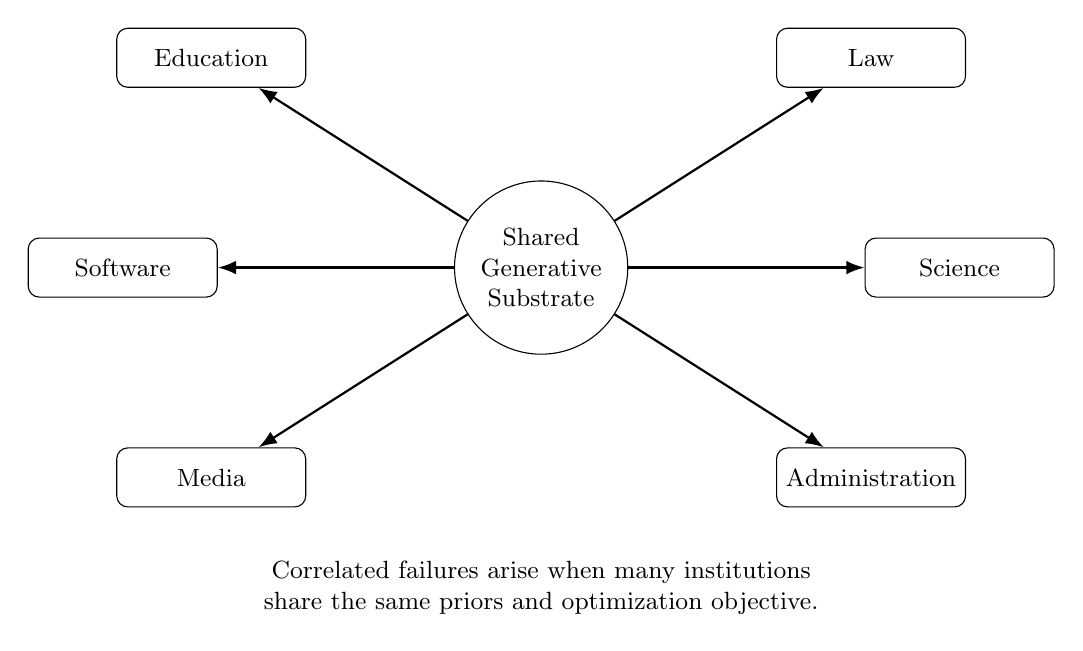
\begin{tikzpicture}[
  node distance=0.9cm,
  box/.style={draw, rounded corners, align=center, minimum width=2.4cm, minimum height=0.75cm, font=\small},
  core/.style={draw, circle, align=center, minimum size=2.2cm, font=\small},
  arrow/.style={-{Latex}, thick}
]
\node[core] (model) {Shared\\Generative\\Substrate};
\node[box, above left=1.5cm and 2.2cm of model] (edu) {Education};
\node[box, above right=1.5cm and 2.2cm of model] (law) {Law};
\node[box, right=3cm of model] (sci) {Science};
\node[box, below right=1.5cm and 2.2cm of model] (admin) {Administration};
\node[box, below left=1.5cm and 2.2cm of model] (media) {Media};
\node[box, left=3cm of model] (soft) {Software};
\foreach \n in {edu,law,sci,admin,media,soft}
  \draw[arrow] (model) -- (\n);
\node[below=2.5cm of model, align=center, font=\small] {Correlated failures arise when many institutions\\share the same priors and optimization objective.};
\end{tikzpicture}
\end{center}

\section{What Honest Development Looks Like}

Aguirre's positive proposal --- redirect from replacement to tool, from general-purpose autonomous agents to specialized purpose-built systems with clearly defined safety criteria and human accountability --- is a necessary but not sufficient condition for improvement. It is necessary because the current trajectory is wrong. It is insufficient because the problems of the metacrisis cannot be addressed by better tools alone. They require reconstruction of the institutional and social conditions that tool use depends on.

The most honest contribution AI development could make to the metacrisis would be a negative one: stop making it worse. Stop building systems optimized for engagement over truth. Stop building attachment architectures that replace intersubjective development with simulated connection. Stop accelerating labor displacement without any serious engagement with what displaced people are supposed to do with their lives. Stop racing toward capabilities that nobody knows how to control.

The positive contribution is more modest than the discourse suggests and more valuable for that modesty. Specialized systems with clearly defined task specifications, external accountability structures, and hard constraints on the scope of their operation have genuine utility in specific domains. AI-assisted formal verification of software can reduce certain categories of vulnerability. Structured tutoring systems with well-defined content domains and limited adaptive scope can improve certain kinds of information transfer. Tools that augment human judgment in well-specified decision contexts, while leaving the judgment firmly with the human, can reduce certain categories of error.

None of this solves the metacrisis. None of it was going to. The metacrisis requires the reconstruction of institutions, the renegotiation of social contracts, the development of new frameworks for managing value pluralism, and the sustained cultivation of the pre-symbolic cognitive capacities that genuine problem-solving requires. These are human tasks. They require intersubjectivity, attentional capacity, institutional trust, and the kind of long-horizon commitment to collective problems that engagement-optimized systems actively erode.

The correct relationship between AI development and the metacrisis is not solution. It is non-interference. Do not make the attentional environment worse. Do not replace intersubjective development with simulations. Do not accelerate institutional disruption without reconstruction. Do not build weapons that remove the friction from violence. Do not race toward capabilities that cannot be governed.

That is a much lower bar than what is being claimed. It is also a bar that current development trajectories are consistently failing to clear.

\bigskip

\noindent\rule{\textwidth}{0.4pt}

\bigskip

\noindent\textit{Flyxion is an independent researcher based in Canada.}

\begin{thebibliography}{99}

\bibitem{Aguirre2024}
Anthony Aguirre.
\textit{Why We Should Build AI Tools, Not AI Replacements}.
Future of Life Institute interviews and lectures, 2024--2025.

\bibitem{Bender2021}
Emily M. Bender, Timnit Gebru, Angelina McMillan-Major, and Shmargaret Shmitchell.
On the Dangers of Stochastic Parrots: Can Language Models Be Too Big?
\textit{Proceedings of the 2021 ACM Conference on Fairness, Accountability, and Transparency}, 2021.

\bibitem{Bowles2016}
Samuel Bowles.
\textit{The Moral Economy: Why Good Incentives Are No Substitute for Good Citizens}.
Yale University Press, 2016.

\bibitem{Carr2010}
Nicholas Carr.
\textit{The Shallows: What the Internet Is Doing to Our Brains}.
W.~W. Norton \& Company, 2010.

\bibitem{Crawford2021}
Kate Crawford.
\textit{Atlas of AI: Power, Politics, and the Planetary Costs of Artificial Intelligence}.
Yale University Press, 2021.

\bibitem{Edgerton2006}
David Edgerton.
\textit{The Shock of the Old: Technology and Global History Since 1900}.
Oxford University Press, 2006.

\bibitem{Floridi2014}
Luciano Floridi.
\textit{The Fourth Revolution: How the Infosphere Is Reshaping Human Reality}.
Oxford University Press, 2014.

\bibitem{Friston2010}
Karl Friston.
The Free-Energy Principle: A Unified Brain Theory?
\textit{Nature Reviews Neuroscience}, 11, 2010.

\bibitem{Geertz1973}
Clifford Geertz.
\textit{The Interpretation of Cultures}.
Basic Books, 1973.

\bibitem{Gigerenzer2007}
Gerd Gigerenzer.
\textit{Gut Feelings: The Intelligence of the Unconscious}.
Viking Press, 2007.

\bibitem{Goodhart1975}
Charles Goodhart.
Problems of Monetary Management: The U.K. Experience.
\textit{Reserve Bank of Australia}, 1975.

\bibitem{Habermas1984}
J\"{u}rgen Habermas.
\textit{The Theory of Communicative Action}.
Beacon Press, 1984.

\bibitem{Han2017}
Byung-Chul Han.
\textit{Psychopolitics: Neoliberalism and New Technologies of Power}.
Verso Books, 2017.

\bibitem{Hayek1945}
Friedrich Hayek.
The Use of Knowledge in Society.
\textit{American Economic Review}, 35(4), 1945.

\bibitem{HomerDixon2000}
Thomas Homer-Dixon.
\textit{The Ingenuity Gap}.
Vintage Canada, 2000.

\bibitem{Illich1971}
Ivan Illich.
\textit{Deschooling Society}.
Harper \& Row, 1971.

\bibitem{Jacobson1995}
Ted Jacobson.
Thermodynamics of Spacetime: The Einstein Equation of State.
\textit{Physical Review Letters}, 75(7), 1995.

\bibitem{Juarrero1999}
Alicia Juarrero.
\textit{Dynamics in Action: Intentional Behavior as a Complex System}.
MIT Press, 1999.

\bibitem{Kahneman2011}
Daniel Kahneman.
\textit{Thinking, Fast and Slow}.
Farrar, Straus and Giroux, 2011.

\bibitem{Klein2007}
Naomi Klein.
\textit{The Shock Doctrine}.
Metropolitan Books, 2007.

\bibitem{Kuhn1962}
Thomas S. Kuhn.
\textit{The Structure of Scientific Revolutions}.
University of Chicago Press, 1962.

\bibitem{Lanier2018}
Jaron Lanier.
\textit{Ten Arguments for Deleting Your Social Media Accounts Right Now}.
Henry Holt and Company, 2018.

\bibitem{Latour1987}
Bruno Latour.
\textit{Science in Action}.
Harvard University Press, 1987.

\bibitem{Luhmann1995}
Niklas Luhmann.
\textit{Social Systems}.
Stanford University Press, 1995.

\bibitem{McLuhan1964}
Marshall McLuhan.
\textit{Understanding Media: The Extensions of Man}.
McGraw-Hill, 1964.

\bibitem{Meadows2008}
Donella Meadows.
\textit{Thinking in Systems}.
Chelsea Green Publishing, 2008.

\bibitem{Merton1968}
Robert K. Merton.
The Matthew Effect in Science.
\textit{Science}, 159(3810), 1968.

\bibitem{Mumford1967}
Lewis Mumford.
\textit{The Myth of the Machine}.
Harcourt Brace Jovanovich, 1967.

\bibitem{Ono2025}
Ken Ono.
\textit{Why This Is the Most Exciting Time to Be Human}.
Public lecture and interview transcript, 2025.

\bibitem{Postman1985}
Neil Postman.
\textit{Amusing Ourselves to Death}.
Penguin Books, 1985.

\bibitem{Russell2019}
Stuart Russell.
\textit{Human Compatible: Artificial Intelligence and the Problem of Control}.
Viking Press, 2019.

\bibitem{Shannon1948}
Claude Shannon.
A Mathematical Theory of Communication.
\textit{Bell System Technical Journal}, 27, 1948.

\bibitem{Simon1971}
Herbert Simon.
Designing Organizations for an Information-Rich World.
In \textit{Computers, Communication, and the Public Interest}, 1971.

\bibitem{Turkle2011}
Sherry Turkle.
\textit{Alone Together}.
Basic Books, 2011.

\bibitem{Tversky1974}
Amos Tversky and Daniel Kahneman.
Judgment Under Uncertainty: Heuristics and Biases.
\textit{Science}, 185(4157), 1974.

\bibitem{Weizenbaum1976}
Joseph Weizenbaum.
\textit{Computer Power and Human Reason}.
W.~H. Freeman, 1976.

\bibitem{Wiener1950}
Norbert Wiener.
\textit{The Human Use of Human Beings}.
Houghton Mifflin, 1950.

\bibitem{Winner1977}
Langdon Winner.
\textit{Autonomous Technology}.
MIT Press, 1977.

\bibitem{Zuboff2019}
Shoshana Zuboff.
\textit{The Age of Surveillance Capitalism}.
PublicAffairs, 2019.

\end{thebibliography}

\end{document}
